\documentclass[a4paper,german,12pt,smallheadings]{scrartcl}
\usepackage[T1]{fontenc}
\usepackage[utf8]{inputenc}
\usepackage{babel}
\usepackage{tikz}
\usepackage{geometry}
\usepackage{amsmath}
\usepackage{amssymb}
\usepackage{float}
\usepackage{cancel}
%\usepackage{wrapfig}
\usepackage[thinspace,thinqspace,squaren,textstyle]{SIunits}
\restylefloat{table}
\geometry{a4paper, top=15mm, left=20mm, right=40mm, bottom=20mm, headsep=10mm, footskip=12mm}
\linespread{1.5}
\setlength\parindent{0pt}
\begin{document}
\begin{center}
\bfseries % Fettdruck einschalten
\sffamily % Serifenlose Schrift
\vspace{-40pt}
Elektrodynamik und Optik, Sommersemester 2013, 6/7. Blatt \\
Markus Fenske und Luis Herrmann, Tutor: Dr. Marko Wietstruk / Paul Stoll
\vspace{-10pt}
\end{center}
\section*{Aufgabe 1}
Das Biot-Savart-Gesetz lautet:

\begin{equation}
  \vec{B}(\vec{r}) = \frac{\mu_0 I}{4 \pi} \int_{\text{Leiter}} \frac{(\vec{r} - \vec{r'}) \times \vec{ds}}{|\vec{r}-\vec{r'}|^3}
\end{equation}

Da hier das Magnetfeld im Ursprung berechnet werden soll, ist:


\begin{equation}
  \vec{B} = \frac{\mu_0 I}{4 \pi} \int_{\text{Leiter}} \frac{(-\vec{r'}) \times \vec{ds}}{|\vec{r'}|^3}
\end{equation}

$\vec{r'}$ ist der der Vektor zum jeweiligen Punkt auf dem Leiter, während
$\vec{ds}$ entlang des Leiters zeigt. Für das gerade Leiterstück ist $\vec{ds}$
also parallel zu $\vec{r}$, womit $\vec{r} \times \vec{ds} = \vec{0}$. Das
gerade Stück kann also vernachlässigt werden.

\begin{equation}
  \vec{B} = \frac{\mu_0 I}{4 \pi} \int_{\text{Bogen}} \frac{(-\vec{r'}) \times \vec{ds}}{|\vec{r'}|^3}
\end{equation}

Auf dem Kreisbogen steht $\vec{ds}$ senkrecht auf $\vec{r}$. Damit gilt dann
$-\vec{r'} \times \vec{ds} = -\widehat{z} (r' ds)$:

\begin{align}
  \vec{B} &= \frac{\mu_0 I}{4 \pi} \int_{\text{Bogen}} -\widehat{z} \frac{r' ds}{r'^3} \\
  \vec{B} &= \frac{\mu_0 I}{4 \pi} \int_{\text{Bogen}} -\widehat{z} \frac{1}{r'^2} ds \\
\end{align}

Sei nun $R$ der Radius des Kreises, dann ist $|\vec{r'}| = R$. Und somit:

\begin{align}
  \vec{B} = -\frac{\mu_0 I}{4 \pi R^2} \widehat{z}\int_{\text{Bogen}} ds \\
\end{align}

Der Kreis hat den Umfang $2 \pi R$, der Halbkreis dementsprechend die Länge
$\pi R$. Das führt zu:

\begin{align}
  \vec{B} = -\frac{\mu_0 I}{4 \pi R^2} \widehat{z} \pi R \\
\end{align}

Und zusammengefasst:

\begin{equation}
  \vec{B} = -\frac{\mu_0 I}{4 \pi R} \widehat{z}
\end{equation}

Da die $z$-Achse aus der Oberseite des Aufgabenblattes herausragt, stimmt dies
auch mit der Rechte-Faust-Regel überein.

\section*{Aufgabe 2}

\begin{figure}[H]
  \begin{center}
    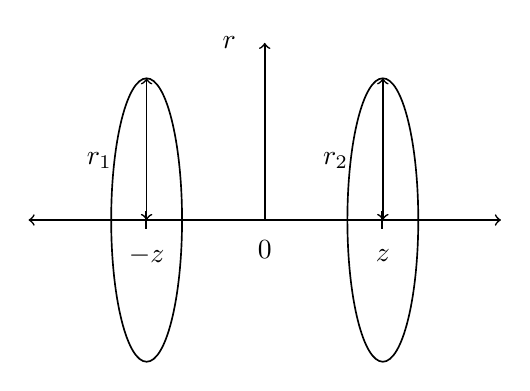
\begin{tikzpicture}[scale=1.5]
      \draw[semithick] (1.0,1.5) ellipse (0.3 and 1.2);% left coil
      \draw[<->,semithick] (1.0,1.5) -- (1.0,2.7); % left radius
      \draw (0.6,2) node {$r_1$}; % left radius text

      \draw[semithick] (3.0,1.5) ellipse (0.3 and 1.2);% right coil
      \draw[<->,semithick] (3.0,1.5) -- (3.0,2.7); % right radius
      \draw (2.6,2) node {$r_2$}; % right radius text

      \draw[->,semithick] (2,1.5) -- (2,3); % r axis
      \draw (1.7,3) node {$r$}; % r axis beschriftung
      \draw (2,1.25) node {$0$}; % ursprung

      \draw[<-|,semithick] (0,1.5) -- (1,1.5);
      \draw[-,semithick] (1,1.5) -- (2,1.5);
      \draw[-|,semithick] (2,1.5) -- (3,1.5);
      \draw[->,semithick] (3,1.5) -- (4,1.5);

      \draw (1,1.2) node {$-z$};
      \draw (3,1.2) node {$z$};
    \end{tikzpicture}
  \end{center}
  \caption{Helmholtzspule}
\end{figure}

Gegeben seien zwei kurze Spulen mit den identischen Radien $r = r_1 = r_2$ und
eine identischen Anzahl an Windungen $N$ an den Positionen $z$ und $-z$. Das
Magnetfeld wird im Zentrum des Aufbaus (also im Ursprung) gemessen und ergibt
sich als Überlagerung der Magnetfelder der beiden Spulen.

Das Magnetfeld einer Leiterschleife ist aus den Vorlesungsunterlagen bekannt,
daher verzichten wir hier auf eine Herleitung. Die Spulen seien Überlagerungen
von jeweils $N$ Leiterschleifen. Daraus folgt für die Magnetfelder:

\begin{align*}
  B = B_1 + B_2 &= \frac{I\mu_0 N}{2} \left(\frac{r^2}{(r^2 + z^2)^{3/2}} + \frac{r^2}{(r^2 + (-z)^2)^{3/2}}\right) \\
            &= I\mu_0 N \left(\frac{r^2}{(r^2 + z^2)^{3/2}}\right)
\end{align*}

Die erste Ableitung lautet:

\begin{align*}
  \frac{\partial B}{\partial z} &= I\mu_0 N r^2 \left(-\frac{3}{2}\right) \cdot 2z \cdot \frac{1}{(r^2 + z^2)^{5/2}} \\
                                &= I\mu_0 N \frac{-3zr^2}{(r^2 + z^2)^{5/2}}
\end{align*}

Die zweite Ableitung lautet:

\begin{align*}
  \frac{\partial^2 B}{\partial z^2} &= -I\mu_0 N \cdot 3 r^2 \frac{\partial}{\partial z} \frac{z}{(r^2 + z^2)^{5/2}} \\
                                    &= -I\mu_0 N \cdot 3 r^2 \left(\frac{1}{(r^2 + z^2)^{5/2}} - \frac{5z^2}{(r^2+z^2)^{7/2}}\right) \\
                                    &= -I\mu_0 N \cdot 3 r^2 \frac{1}{(r^2 + z^2)^{7/2}} \left( (r^2+z^2) - 5z^2 \right) \\
                                    &= -I\mu_0 N \cdot 3 r^2 \frac{1}{(r^2 + z^2)^{7/2}} \left( r^2 - 4z^2 \right) \\
\end{align*}

Die zweite Ableitung nun weiter zusammenzufassen wäre Verschwendung von
teurer Drucktinte. Wir suchen $\partial_z^2 B \overset{!}{=} 0$. Obiger Ausdruck
muss also null werden. Dies passiert offensichtlich nur dann, wenn die innerste
Klammer null wird.

\begin{align*}
  &r^2 - 4z^2 \overset{!}{=} 0 \\
  \Leftrightarrow\quad & r^2 = 4z^2 \\
  \Leftrightarrow\quad & r = \pm 2z \\
  \Rightarrow\quad &z = \pm\frac{r}{2}
\end{align*}

Die Abstände $z$ müssen also jeweils das Halbe des Spulenradius betragen,
damit das Feld möglichst homogen wird. Das $\pm$ bedeutet nur, dass die Spulen
prinzipiell vertauschbar sind. Der Abstand zwischen den Spulen muss also genau
dem Radius der Spulen entsprechen.

\section*{Aufgabe 3}

\begin{equation}
  \vec{p}_m = I \vec{A}
\end{equation}

Das magnetische Dipolmoment ist $p_m = I \cdot \vec{A}$. Dabei ist $I$ der
Strom und $\vec{A}$ die Flächennormale der Kreisbahn. Da diese parallel zum
Drehmoment, genau wie zum Drehimpuls ist, reicht es, hier mit Beträgen zu
arbeiten.

\begin{equation}
  p_m = I A
\end{equation}

Für $I$ gilt $I = \frac{dQ}{dt}$. Das Elektron kommt auf seiner Kreisbahn mit
dem Radius $r$ genau einmal pro Umlaufzeit $t$ am Ausgangspunkt vorbei. Der
Strom ist also

\begin{equation}
  I = \frac{-e}{t}
\end{equation}

Die Umlaufzeit auf der Kreisbahn $s$ mit der Geschwindigkeit $v$ ist:

\begin{equation}
  t = \frac{s}{v} = \frac{2 \pi r}{v}
\end{equation}

Eingesetz in die Ausgangsgleichung:

\begin{equation}
  p_m = \frac{-e}{2 \pi r} v A
\end{equation}

Die Kreisfläche ist $A = \pi r^2$. Eingesetzt:

\begin{equation}
  p_m = \frac{-e}{2 \pi r} v \pi r^2 = \frac{-e}{2} v r
\end{equation}

Mit dem Impuls $p = mv$ erhält man:

\begin{equation}
  p_m = \frac{-e}{2m} p r
\end{equation}

Und mit dem Drehimpulsbetrag $L = pr$:

\begin{equation}
  p_m = \frac{-e}{2m} L
\end{equation}

Wenn wir nun $L = \hbar$ einsetzen erhalten wir:

\begin{equation}
  p_m = \frac{-e}{2m_e} \hbar \approx -9{,}274 \cdot 10^{-24} \;\joule\per\tesla
\end{equation}

\section*{Aufgabe 4}
\subsection*{Teil a}

Nach Austritt aus dem Plattenkondensator hat die Geschwindigkeit des Elektrons zusätzlich zur x-Komponente eine y-Komponente erhalten. Um den Betrag der y-Komponente zu ermitteln überlegen wir uns, dass eine konstante Beschleunigung in y-Richtung $a_y$ auf das Teilchen wirkt:
\begin{equation*}
a_y=\frac{v_y}{t} \quad \Leftrightarrow \quad v_y=a_yt
\end{equation*}

Aus dem 2. Newtonschen Gesetz folgt:
\begin{equation*}
F=a \cdot m \quad \Rightarrow \quad F_y=a_ym \quad \Leftrightarrow \quad a_y=\frac{F_y}{m}
\end{equation*}

Die Kraft in y-Richtung ergibt sich aus dem homogenen elektrischen Feld zwischen den Kondensatorplatten:
\begin{equation*}
E_y=\frac{F_y}{q} \quad \Leftrightarrow \quad F_y=E_yq
\end{equation*}

Eingesetzt in den Ausdruck für $a_y$:
\begin{equation*}
a_y=\frac{E_yq}{m}
\end{equation*}

...und eingesetzt im Ausdruck für $v_y$:
\begin{equation*}
v_y=\frac{E_yq}{m} \cdot t
\end{equation*}

Dabei ist t der Zeitraum zwischen Eintritt des Elektrons in die Kondensatorplatten und Austritt.  Dieser lässt sich über die x-Komponente der Geschwindigkeit $v_x$ und die Länge der Kondensatorplatten $x$ ermitteln:
\begin{equation*}
v_x=\frac{x}{t} \quad \Leftrightarrow \quad t=\frac{x}{v_x}
\end{equation*}

Wir erhalten somit:
\begin{equation*}
v_y=\frac{E_yqx}{mv_x}
\end{equation*}

Sobald das Elektron in das Magnetfeld eintritt, wirkt auf dieses die Kraft:
\begin{equation*}
\vec{F}=q\vec{v_y} \times \vec{B} \quad \text{,wegen $\vec{v_y} \perp \vec{B}$ betragsweise:} \quad F=qv_yB
\end{equation*}

Gleichsetzen mit der Zentripetalkraft der Drehbewegung des Elektrons im Magnetfeld:
\begin{equation*}
qv_yB=\frac{mv_y^2}{r} \quad \Leftrightarrow \quad r=\frac{m v_y}{qB}=\frac{E\cancel{q}x}{\cancel{m}v_x} \cdot \frac{\cancel{m}}{\cancel{q}B}=\frac{Ex}{Bv_x}
\end{equation*}

Einsetzen:
\begin{align*}
r=\frac{10^4V/m \cdot 0.05m}{10^{-2}T \cdot 10^7m/s} = 5 \cdot 10^{-3}m=5mm
\end{align*}

\subsection*{Teil b}
Für die Zyklotronperiode haben wir den Ausdruck gefunden:
\begin{equation*}
\tau=\frac{2\pi m}{qB}
\end{equation*}

Dann ist der Abstand zwischen zwei Windungen der Schraubenkurve gerade:
\begin{equation*}
s=v_x\tau = \frac{2 \pi m v_x}{qB}
\end{equation*}

Mit $q=e$ und $m=m_e$(Masse des Elektrons):
\begin{equation*}
\quad s=\frac{2 \pi m_e v_x}{eB}
\end{equation*}

Einsetzen:
\begin{equation*}
s=\frac{2\pi \cdot 9,109 382\cdot 10^{-31}kg \cdot 10^7 m/s}{1.6022 \cdot 10^{-19}C \cdot 10^{-2}T} \approx 0.0357m
\end{equation*}

\section*{Aufgabe 5}
Wir gehen davon aus, dass mit $B_v$ die Komponente des Erdmagnetfeldes ist, die senkrecht zum Geschwindigkeitsvektor $v$ des Flugzeugs steht. Dann gilt nämlich:

\begin{equation*}
U_H=v_dB_vd \quad \text{;sei $v_d$ die Driftgeschwindigkeit der Ladungen}
\end{equation*}

...doch welche Ladungen, wenn durch das Flugzeug gar kein Strom hindurch fließt? Tatsächlich befinden sich in der Luft ionisierte Teilchen. Wenn das Flugzeug mit der Geschwindigkeit $v$ relativ zur Luft fliegt, ist dies äquivalent zu einem elektrischen Strom, bei dem die Ladungen eine Driftgeschwindigkeit von $v=v_d$ haben. \\

Durch das Erdmagnetfeld kommt es zur einer Auslenkung der Teilchen und zum Aufbau einer Spannung entlang der Tragflächen des Flugzeugs. Sei $d=b$ und b die Spannweite des Flugzeugs:

\begin{equation*}
U_H=vB_vb
\end{equation*}

Einsetzen:
\begin{equation*}
U_H=\frac{980m/s}{3.6}\cdot 0.47 \cdot 10^{-4}T \cdot 54m =0.6909V
\end{equation*}

...diese Spannung würde nicht einmal ausreichen, um eine LED zu betreiben.

\section*{Aufgabe 6}
\subsection *{Teil a}

Für sehr lange, gerade Leiter haben wir in der Vorlesung das Magnetfeld wie folgt ausgedrückt:
\begin{equation*}
B_0=\frac{\mu_0 I_0}{2\pi r}
\end{equation*}

...sei r der Abstand senkrechte Abstand eines Punktes zum Leiter. Zu berücksichtigen ist, dass sich die Drähte in einem homogenen Isolator befinden, sodass für das gesamte Magnetfeld gilt:
\begin{equation*}
B=\mu_r  = \frac{\mu_r \mu_0 I_0}{2\pi r}
\end{equation*}

Also sind:
\begin{equation*}
B_1=\mu_r  = \frac{\mu_r \mu_0 I_1}{2\pi r_1} \quad B_2=\mu_r  = \frac{\mu_r \mu_0 I_2}{2\pi r_2}
\end{equation*}

Zur Lösung des Problems wählen wir das Koordinatensystem so, dass $r_1=\frac{d}{2}$ und $r_2=-\frac{d}{2}$. Durch Superposition beider Magnetfelder erhalten wir das Gesamtmagnetfeld in der Mitte:
\begin{equation*}
B_{ges}=B_1+B_2= \frac{\mu_r \mu_0 I_1}{\pi d}- \frac{\mu_r \mu_0 I_2}{\pi d}
\end{equation*}

Mit $I_2=-I_1$:
\begin{equation*}
B_{ges}=\frac{\mu_r \mu_0 I_1}{\pi d}+ \frac{\mu_r \mu_0 I_1}{\pi d}=\frac{2\mu_r \mu_0 I_1}{\pi d}
\end{equation*}

Einsetzen:
\begin{equation*}
B_{ges}=\frac{2\cdot 120 \cdot 4\pi \cdot 10^{-7} N/A^2 \cdot 40A}{\pi \cdot 0.04m} =0.096T
\end{equation*}

\subsection*{Teil b}

In der Vorlesung hergeleitet:
\begin{align*}
\frac{F}{l}=\frac{\mu_0 I_1 I_2}{2 \pi r}
\end{align*}

Unter Berücksichtigung des Isolators, sowie mit $I_1=-I_2$ und  mit $\frac{d}{2}$:
\begin{align*}
\frac{F}{l}=\frac{\mu_r \mu_0 -I_1^2}{\pi d}
\end{align*}

Einsetzen:
\begin{align*}
\frac{F}{l}=-\frac{120 \cdot 4\pi \cdot 10^{-7}N/A^2 \cdot (40A)^2}{\pi \cdot 0.04}=1.92N
\end{align*}

\section*{Aufgabe 7}
\subsection*{Teil a}
Für das Magnetfeld einer langen Spule gilt

\begin{equation}
  B = \mu_0 \mu_r \frac{n}{l} I
\end{equation}

In diesem Fall:

\begin{align*}
  B \approx 60 \;\milli\tesla
\end{align*}

\subsection*{Teil b}
Aus obiger Gleichung ist klar, dass $I$ mit dem Faktor $1200$ multipliziert
werden muss, wenn $\mu$ durch $1200$ dividiert wird. Dementsprechend muss dann
$I = 1200 \cdot 20\;\milli\ampere = 24\;\ampere$ sein.


\section*{Aufgabe 8}
\subsection*{Teil a}

Offensichtlich gilt:
\begin{equation*}
p_M=p_m \cdot n \quad \text{; sei $n$ die Anzahl der Atome im Würfel}
\end{equation*}

Weiterhin gilt:
\begin{align*}
V=a^3\\
\frac{M}{V}=\rho \quad \Leftrightarrow \quad M=\rho V = \rho a^3
\end{align*}

Für die Anzahl der Atome im Würfel gilt:
\begin{equation*}
M=m\cdot n \quad \Leftrightarrow \quad n=\frac{M}{m}
\end{equation*}

Einsetzen der obigen Gleichung liefert:
\begin{equation*}
M=\frac{\rho a^3}{m} \quad \Rightarrow \quad p_M=\frac{p_m \rho a^3}{m}
\end{equation*}

Einsetzen:
\begin{equation*}
p_M=\frac{1.8 \cdot 10^{-23}Am^2 \cdot 7874 kg/m^3 \cdot (0.012m)^3}{55.845 \cdot 1.660 \cdot 10^{-27}kg} \approx 2.6419 Am^2
\end{equation*}

\subsection*{Teil b}
siehe Anhang für Skizze\\

Da es in Ferromagneten Felder mit einheitlichem magnetischem Moment gibt, die sogenannten "Weiß'schen Bezirke", verändern unter Einwirkung eines äußeren Magnetfeldes ganze Felder ihr magnetisches Moment, (dies äußert sich in einer graduellen Schrumpfung der Weiß'schen Bezirke mit zunehmender angelegter Feldstärke) und die magnetische Sättigung lässt sich bei ausreichend starken Magnetfeldern mit hoher Wahrscheinlichkeit erreichen.
Bei Diamagneten hingegen muss jedes Atom einzeln ausgerichtet werden. Selbst bei hohen Feldstärken bleiben jedoch immer noch Atome übrig, deren magnetisches Moment nicht dem gerade angelegten Magnetfeld entsprechend ausgerichtet ist. Die magnetische Sättigung ist so schwerer zu erreichen.

\subsection*{Teil c}

Das Gesamtmagnetfeld ergibt sich bei Ferromagnetismus wie folgt:
\begin{equation*}
B_{ges}=\underbrace{B_{aus}}_{ausseres Magnetfeld}+\underbrace{\mu_0M}_{induziertes Magnetfeld}
\end{equation*}

Also ist:
\begin{align*}
B_{ind}=\mu_0M=\cancel{\mu_0} \cdot \frac{B_{aus} \mathcal{X}_{mag}}{\cancel{\mu_0}}=B_{aus}\mathcal{X}_{mag}=\mu_0H_{mag}\mathcal{X}_{mag}
\end{align*}

Einsetzen:
\begin{align*}
B_{ind}=4\pi \cdot 10^{-7} N/A^2 \cdot 180 A/m \cdot 500 \approx 0.1131T
\end{align*}

\subsection*{Teil d}

Die zugehörige Magnetisierung ist einfach:
\begin{equation*}
M=\frac{B_{aus}\mathcal{X}}{\mu_0}=H_{aus} \mathcal{X}_{aus}
\end{equation*}

Einsetzen:
\begin{equation*}
M=180A/m \cdot 500=90kA/m
\end{equation*}

\end{document}
